\chapter{The GEM and CSC Data Acquisition Systems}
\label{chap:II-2-daq}

  The installation of GEM detectors in CMS and the integration with the CSCs require the development of a new DAQ system for the GE1/1 project. The understanding of the structure of both the GEM and CSC readout chains as well as the common CMS central DAQ is of importance in the scope of this thesis. To this end, all three systems are presented in details in the sections that follow. \\

  \section{The GE1/1 Data Acquisition System}

    The architecture of the GE1/1 DAQ system is represented in Figure \ref{fig:II-2-daq-gem-system}. It is divided into two sectors: the on-detector electronics on the left in charge of the managment of the detector, and the off-detector electronics on the right responsable for the data handling and the connection to the central DAQ. The two sectors are separated by a few douzen meters and connected through optical fibres. \\

    \begin{figure}[h!]
      \centering
      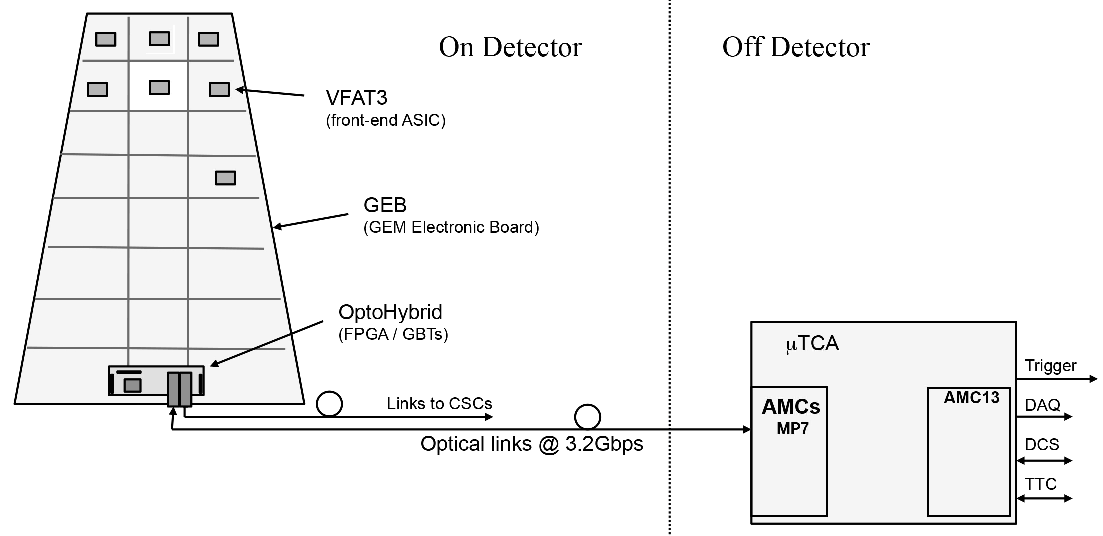
\includegraphics[width=0.7\textwidth]{img/II-2-daq/gem-system.pdf}
      \caption{??? \cite{Colaleo:2021453}.}
      \label{fig:II-2-daq-gem-system}
    \end{figure}

    The on-detector electronics focuses on the control and readout of the VFAT3 Application Specific Integrated Circuit (ASIC) which connects to the strips of the chamber and digitizes the data. The GEM Electronics Board (GEB), on which the VFAT3s are plugged in, then routes the signals to the OptoHybrid (OH) which acts as concentrator board and communication relay for the 24 VFAT3s. The communication with the off-detector system is performed through the GigaBit Tranciever (GBT) chipset and the Versatil Link installed on the OH. Both projects are led by CERN and provide radiation hard tools for LHC experiments. \\

    On the off-detector side, the Micro Telecommunications Computing Architecture (microTCA, MTCA, or $\mu$TCA) \cite{PICMG} crate standard is used to power and monitor the Advanced Mezzanine Cards (AMCs) which provide the ressources to communicate with the on-detector electronics. Links from multiple OHs are concentrated on one MP7 AMC which formats the data and transfers it to the CMS AMC13 mezzanine. The AMC13 is the link between the microTCA crate and the central DAQ of CMS which provides the clocking, trigger, and control over the system. The control of the DAQ chain is performed from a XDAQ application using the IPBus protocol over ethernet. 

    \subsection{The VFAT3 ASIC}

    \begin{figure}[h!]
      \centering
      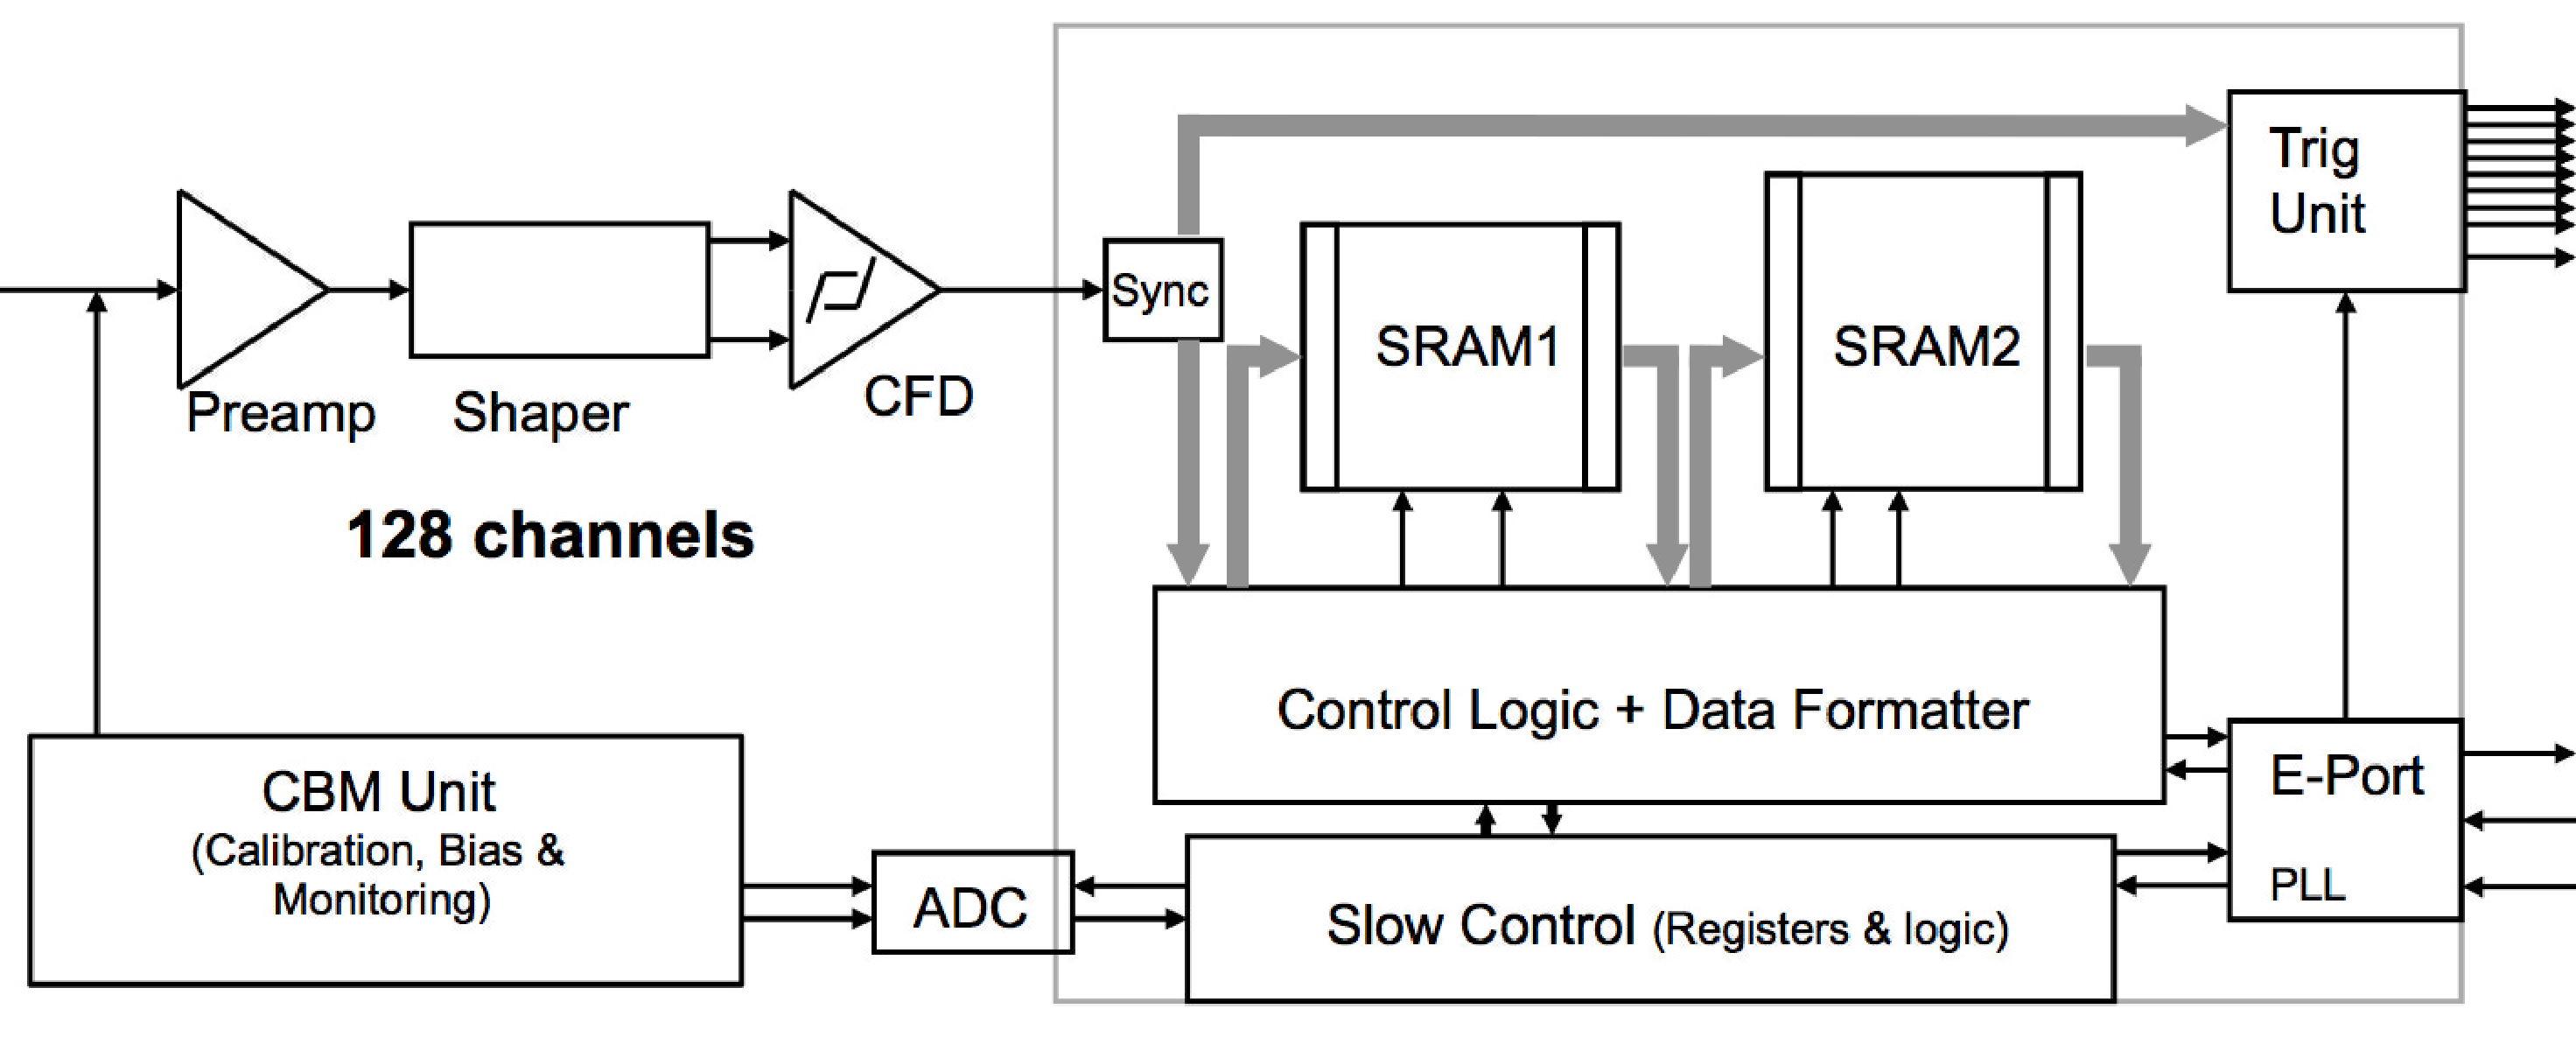
\includegraphics[width=\textwidth]{img/II-2-daq/vfat3.pdf}
      \caption{??? \cite{Colaleo:2021453}.}
      \label{fig:II-2-daq-vfat3}
    \end{figure}

    \begin{figure}[h!]
      \centering
      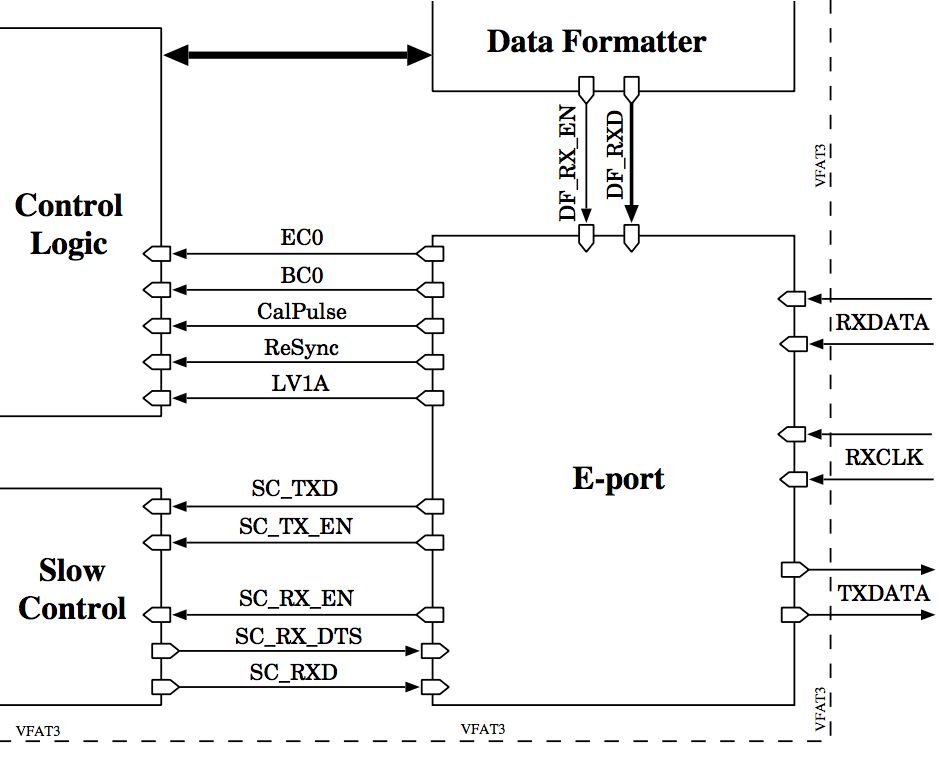
\includegraphics[width=0.8\textwidth]{img/II-2-daq/vfat3-eport.png}
      \caption{??? \cite{Colaleo:2021453}.}
      \label{fig:II-2-daq-vfat3-eport}
    \end{figure}

    \subsection{The GEM Electronics Board}

    \subsection{The OptoHybrid}

    \subsection{The GBT and Versatil Link}

    \subsection{The microTCA Standard}

    \subsection{The MP7 Advanced Mezzanine Card}

    \subsection{The AMC13}

    \subsection{The IPBus Protocol}

    \subsection{The XDAQ Application}

  \section{The CSC Data Acquisition System}

  \section{The CMS Central Data Acquisition System}
